\documentclass[12pt,a4paper]{amsart}

\synctex = 1

\DeclareMathAlphabet{\mathpzc}{OT1}{pzc}{m}{it}

\def\Bb{\mathbb{B}}
\def\C{\mathbb{C}}
\def\E{\mathbb{E}}
\def\F{\mathbb{F}}
\def\Hh{\mathbb{H}}
\def\K{\mathbb{K}}
\def\N{\mathbb{N}}
\def\P{\mathbb{P}}
\def\Q{\mathbb{Q}}
\def\R{\mathbb{R}}
\def\Z{\mathbb{Z}}



%A
\DeclareMathOperator{\akte}{akte}
%B
\DeclareMathOperator{\bearbeitet}{bearbeitet}
\DeclareMathOperator{\Black}{Black}
%C
\DeclareMathOperator{\cons}{cons}
%D
\DeclareMathOperator{\deff}{def}
\DeclareMathOperator{\Dom}{Dom}
%E
\DeclareMathOperator{\Einbruch}{Einbruch}
\DeclareMathOperator{\ermittler}{ermittler}
\DeclareMathOperator{\ext}{ext}
%F
%G
\DeclareMathOperator{\gdw}{gdw}
%H
\DeclareMathOperator{\HB}{HB}
%I
%J
%K
\DeclareMathOperator{\Konst}{Konst}
%L
\DeclareMathOperator{\wle}{le}
\DeclareMathOperator{\ltdermittler}{ltdermittler}
%M
\DeclareMathOperator{\Mulder}{Mulder}
%N
\DeclareMathOperator{\Name}{Name}
%O
\DeclareMathOperator{\offen}{offen}
%P
\DeclareMathOperator{\Pathologie}{Pathologie}
\DeclareMathOperator{\Pred}{Pred}
%Q
%R
%S
\DeclareMathOperator{\Skinner}{Skinner}
\DeclareMathOperator{\Skully}{Skully}
\DeclareMathOperator{\Sonderermittler}{Sonderermittler}
%T
%U
%V
\DeclareMathOperator{\Verwaltung}{Verwaltung}
%X
%Z

\def\fspace{\rule{0.5cm}{0cm}}
\theoremstyle{definition}
\newtheorem{aufgabe1}{Aufgabe}

\usepackage{amsmath,amsthm,amssymb}
\usepackage[utf8]{inputenc}
\usepackage{wasysym}
\usepackage{stmaryrd}
\usepackage{nicefrac}
\usepackage{listings}
\usepackage{pictex}
\usepackage{color}
\usepackage{graphicx}
\usepackage{german}


%%%%%%%%%%%%%%%%%%%%%%%%%%%%%%%%%%%%%%%%%%%%%%%%%%%%%%%%%%%%%%%%%%%%%%%

\begin{document}

\title{Blatt 6}

\author{Daniel Schmidt \& Pamela Fleischmann}

\maketitle

\begin{aufgabe1}

\end{aufgabe1}

\begin{aufgabe1}
Betrachte folgendes Datalog-Programm:\\
$p(a,b,c,d,e,f). p(a,a,b,b,c,c). p(a,a,a,b,b,c). p(c,c,c,b,b,a).$\\
$r_1= q(U,V,W,X,Y,Z) :- p(U,V,W,X,Y,Z).$\\
$r_2=q(U,V,W,X,Y,Z) :- q(Z,U,V,W,X,Y).$\\
$r_3=q(X,Y,Z,U,V,W) :- q(U,V,X,W,Y,Z), q(W,Y,Z,U,V,X).$\\
$r_4=r(X,Y,Z) :- q(X,Y,X,Z,X,Y).$\\
Sei weiter $r(a,b,c)$ ein Ziel. Dann hat ein Beweisbaum zu $r(a,b,c)$ die folgende Form
\begin{center}
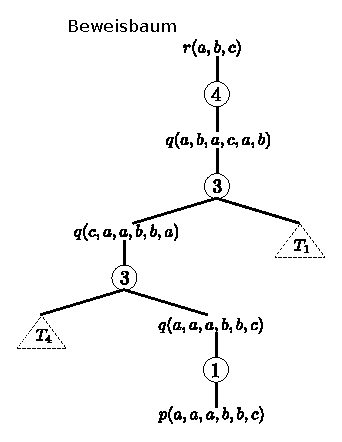
\includegraphics[]{tree.eps}
\end{center}
mit den Unterbäumen
\begin{center}
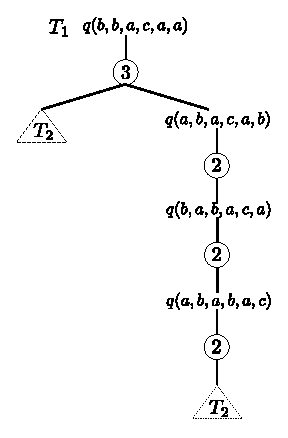
\includegraphics[]{t1.eps} 
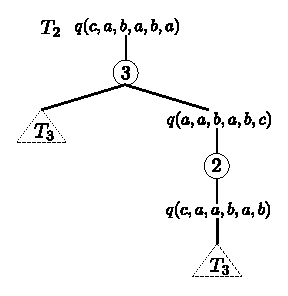
\includegraphics[]{t2.eps}
\end{center}
\begin{center}
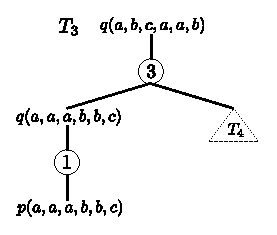
\includegraphics[]{t3.eps}

\includegraphics[]{t4.eps}
\end{center}
\end{aufgabe1}


\begin{aufgabe1}
\begin{verbatim}
dfa(L) :- start(S), transition(S,L).

trans(S1,[A|W]) :- delta(S1,A,S2), transition(S2,W).  
trans(S1,[]) :- final(S1).

start(0).
final(3).
delta(0,a,1).   
delta(0,b,2).
delta(1,a,2).
delta(1,b,0).
delta(2,a,2).
delta(2,b,2).
delta(3,a,4).
delta(3,b,2).
delta(4,a,2).
delta(4,b,0).
\end{verbatim}
$L=(ab)^{\ast}ab(ab)^{\ast}$
\end{aufgabe1}

\end{document}
